% Section 3
% BOSS and voBOSS
\section{BOSS}

\begin{frame}
\frametitle{Succint de Bruijn Graphs - (Bowe, Sadakane, 2012)}
\textcolor{red}{Achievement}: $4+o$(1) bits per edge (independent of k)
\\ \medskip
Inspiration taken from:
\begin{itemize}
	\item BW Transform [Burrows, Wheeler 94]	
	\item XBW Transform [Ferragina et al. 05]
\end{itemize}
\end{frame}

\begin{frame}
\frametitle{Succint de Bruijn Graphs - Three arrays to represent a graph}
Assuming that \textbf{m} is the number of edges of the graph
\begin{enumerate}
	\item take each k-mer and \textbf{sort} them in reverse lexicographical order
	\\ $\Rightarrow$ Array \textbf{Node} - \textcolor{red}{Don't worry we won't store it explicitly}.
	\item store for each node the label of its outgoing edges 
	\\ $\Rightarrow$ Array \textbf{W}
	\item store a bitvector \textbf{L} of size \textbf{m} whose entries are: $L[i] = 1 \Leftrightarrow Node[i] ≠ Node[i+1]$ \\
	i.e.: indicates the range in which Node refers the same node
	\\ $\Rightarrow$ Array \textbf{L}
\end{enumerate}
\end{frame}

\begin{frame}
\frametitle{Succint de Bruijn Graphs - visualising BOSS}
\begin{columns}
	\column{0.5\textwidth}
	\begin{figure}
		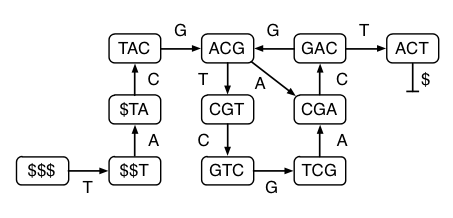
\includegraphics[scale=0.4]{img/sdbg-graph-padded.png}
	\end{figure}
	\column{0.5\textwidth}
	\begin{figure}
		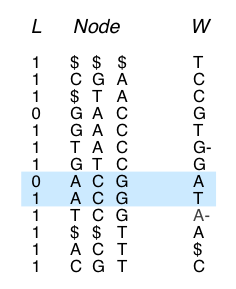
\includegraphics[scale=0.5]{img/sdbg-arrays-1.png}
	\end{figure}
\end{columns}
\end{frame}

\begin{frame}
\frametitle{Optimizing space}
\begin{columns}
	\column{0.5\textwidth}
	Instead of storing the node labels we can save space by just storing the final column of the node labels.
	\\ \medskip
	Since the node labels are sorted, it is equivalent to store an array of first positions. \\ \medskip
	Array \textbf{Node} $\Rightarrow$ Array \textbf{F}
	\column{0.6\textwidth}
	\begin{figure}
		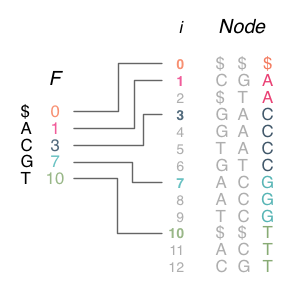
\includegraphics[scale=0.5]{img/f-array.png}
	\end{figure}
\end{columns}
\end{frame}

\begin{frame}
\frametitle{Total space used}
Assuming that our graph has \textbf{m} edges we get:
\begin{enumerate}
	\item Array \textbf{L} $\Rightarrow$ $m$ bits
	\item Array \textbf{W} $\Rightarrow$ $m\ log\ 2^\sigma\ =\ 3\ m$ (in case of DNA alphabet)
	\item Array \textbf{F} $\Rightarrow$ $\sigma\ log\ m\ =\ o(m)$
\end{enumerate}
So total space required is  $4+o$(1) bits per edge. 
\end{frame}



\begin{frame}
\frametitle{Fast travelling across the succint dBG}
Recall that \textbf{DNA sequences can be reconstructed by moving between nodes of the dBG graph}.
\\ \medskip
So we need some way, \textcolor{red}{hopefully fast}, to move through nodes and edges.
\\ \medskip
Thanks to two simple observations derived from how we succintly represented our graph and rank / select queries support for two of our three vectors we will achieve the wished speed of use.
\end{frame}

\begin{frame}
\frametitle{BOSS properties - 1}
\begin{claim}[1]
	All the edges going out from a node are next each other in the representation
\end{claim}
\begin{figure}
	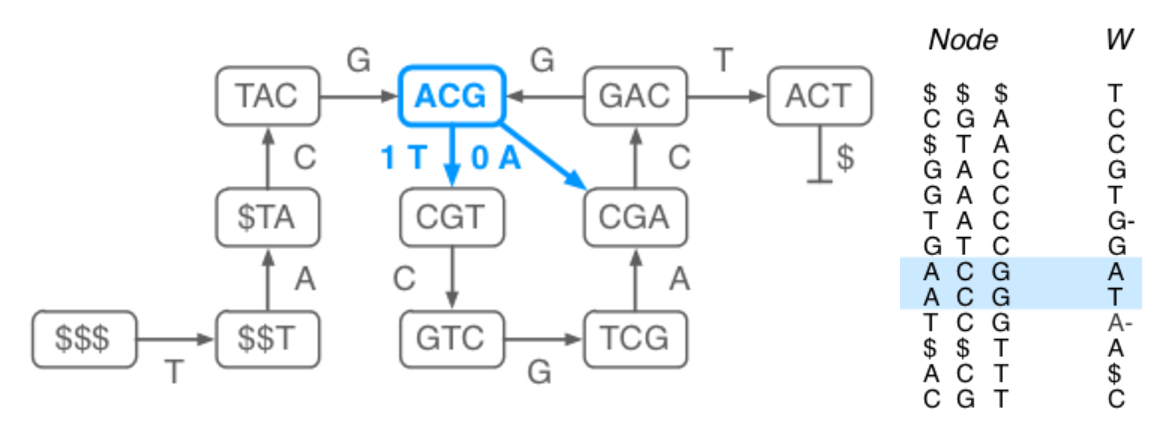
\includegraphics[scale=0.25]{img/claim1.png}
\end{figure}
\end{frame}

\begin{frame}
\frametitle{BOSS properties - 2}
\begin{claim}[2]
	Nodes labels in the last column of \textbf{Node} maintain the same relative order as the edge labels in \textbf{W}.
\end{claim}
\begin{figure}
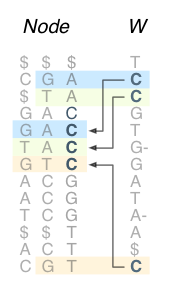
\includegraphics[scale=0.45]{img/claim2.png}
\end{figure}
\end{frame}

\begin{frame}
\frametitle{Some other observations}
\begin{enumerate}
	\item In a dBG every node is defined by its previous k edges.
	\item It may be the case that we need to disambiguate between edges that exit separate nodes but have the same label and enter the same node. (flagged labels in \textbf{W})
	\item Since a 1 in the \textbf{L} vector identifies a unique node,\\ 
	we can use this vector to index nodes (\textbf{HINT}: use $select_1$),\\
	whereas standard array accesses refer to edges.
\end{enumerate}
\end{frame}

\begin{frame}
\frametitle{Basic navigation: going forward and backward}
In order to support some public interface to navigate the graph, we first devise two simple procedures based on rank and select queries to work with edges: 
\begin{itemize}
	\item \textbf{forward(i)}: returns the index of the last edge of the node pointed by edge i.
	\item \textbf{backward(i)}: returns the index of the first edge that points to the node that the edge at i exits. 	
\end{itemize}
\end{frame}


\begin{frame}
\frametitle{Forward}
Thanks to \textbf{Claim 2} following an edge is simply finding the corresponding relatively positioned node. \\
\underline{Example}: \textbf{forward(2)}
\begin{figure}
	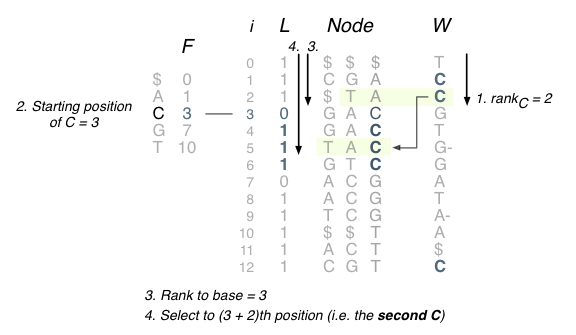
\includegraphics[scale=0.4]{img/fwd.png}
\end{figure}
\end{frame}

\begin{frame}
\frametitle{Backward}
Again thanks to \textbf{Claim 2} following an edge backwardly is equivalent to the corresponding relatively positioned edge. \\
\underline{Example}: \textbf{backward(5)}
\begin{figure}
	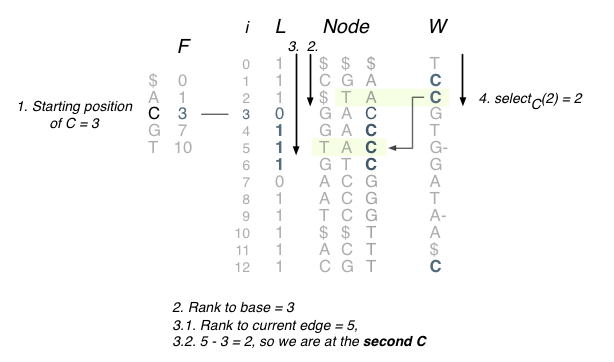
\includegraphics[scale=0.4]{img/bwd.png}
\end{figure}
\end{frame}

\begin{frame}
\frametitle{Supported operations}
At this point we can use \textbf{forward(i)} and \textbf{backward(i)} to support the following operations:
\begin{itemize}
	\item \textbf{outdegree(v)}: \#outgoing edges for node v.\\ $\mathcal{O}$(1) time
	\item \textbf{outgoing(v, c)}: node reached from v through edge labelled c.\\ $\mathcal{O}$(1) time
	\item \textbf{indegree(v)}: \#incoming edges for node v.\\ $\mathcal{O}$(1) time
	\item \textbf{incoming(v, c)}:  predecessor node starting with symbol c, that has an edge to node v.\\ $\mathcal{O}$(k $log\ \sigma$) time
	\item \textbf{label(v)}: complete label of the node v.\\ $\mathcal{O}$(k) time
\end{itemize}
%Note that the parameters to fwd and bwd are index of edges while paramenters for the other operations are node indexes so that we must first select them
\end{frame}

\begin{frame}
\frametitle{Implementing outgoing(v, c)}
Similar to \textbf{forward(i)} but now we want to move starting from a given node v.
\\ \medskip
\underline{Example}: \textbf{outgoing(6, T)}
\begin{figure}
	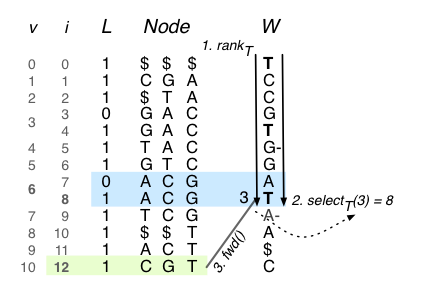
\includegraphics[scale=0.4]{img/outgoing.png}
\end{figure}

\end{frame}

\begin{frame}
\frametitle{Implementing label(v)}
During a traversal we may want to print the node labels out.
\\
We use the position of our node (\textbf{found using select(v)}) as a reverse lookup into \textbf{F} and then we do a series of k backward calls.
\\ \medskip
\underline{Example}: \textbf{label(6)} 
note that in step 1 we do a select(6+1)!
  \begin{columns}
	\column{0.5\textwidth}
	  \begin{figure}
	  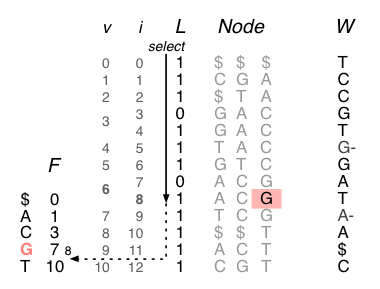
\includegraphics[scale=0.4]{img/label1.png}
	  \end{figure}
	\column{0.5\textwidth}
      \begin{figure}
	   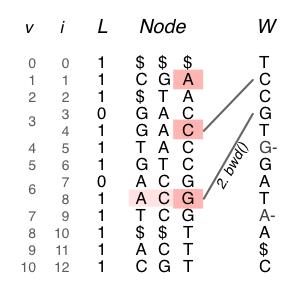
\includegraphics[scale=0.4]{img/label2.png}
      \end{figure}
  \end{columns}
\end{frame}

\begin{frame}
\frametitle{Summarizing the results}
\begin{itemize}
	\item $ m*(2+log\ \sigma +o(1))$ bits, \textcolor{red}{$4m\ +\ o(m)$ bits for DNA}
	\item The size does not depend on k-mer length, so it is effective for large k too.
	\item useful navigation queries are perfomed in constant and in logarithmic time.
\end{itemize}
\end{frame}
